%
% karten.tex -- template for standalon tikz images
%
% (c) 2021 Prof Dr Andreas Müller, OST Ostschweizer Fachhochschule
%
\documentclass[tikz]{standalone}
\usepackage{amsmath}
\usepackage{times}
\usepackage{txfonts}
\usepackage{pgfplots}
\usepackage{csvsimple}
\usetikzlibrary{arrows,intersections,math}
\begin{document}
\def\skala{1}
\begin{tikzpicture}[>=latex,thick,scale=\skala]

\definecolor{darkgreen}{rgb}{0,0.6,0}

\node at (0,0) {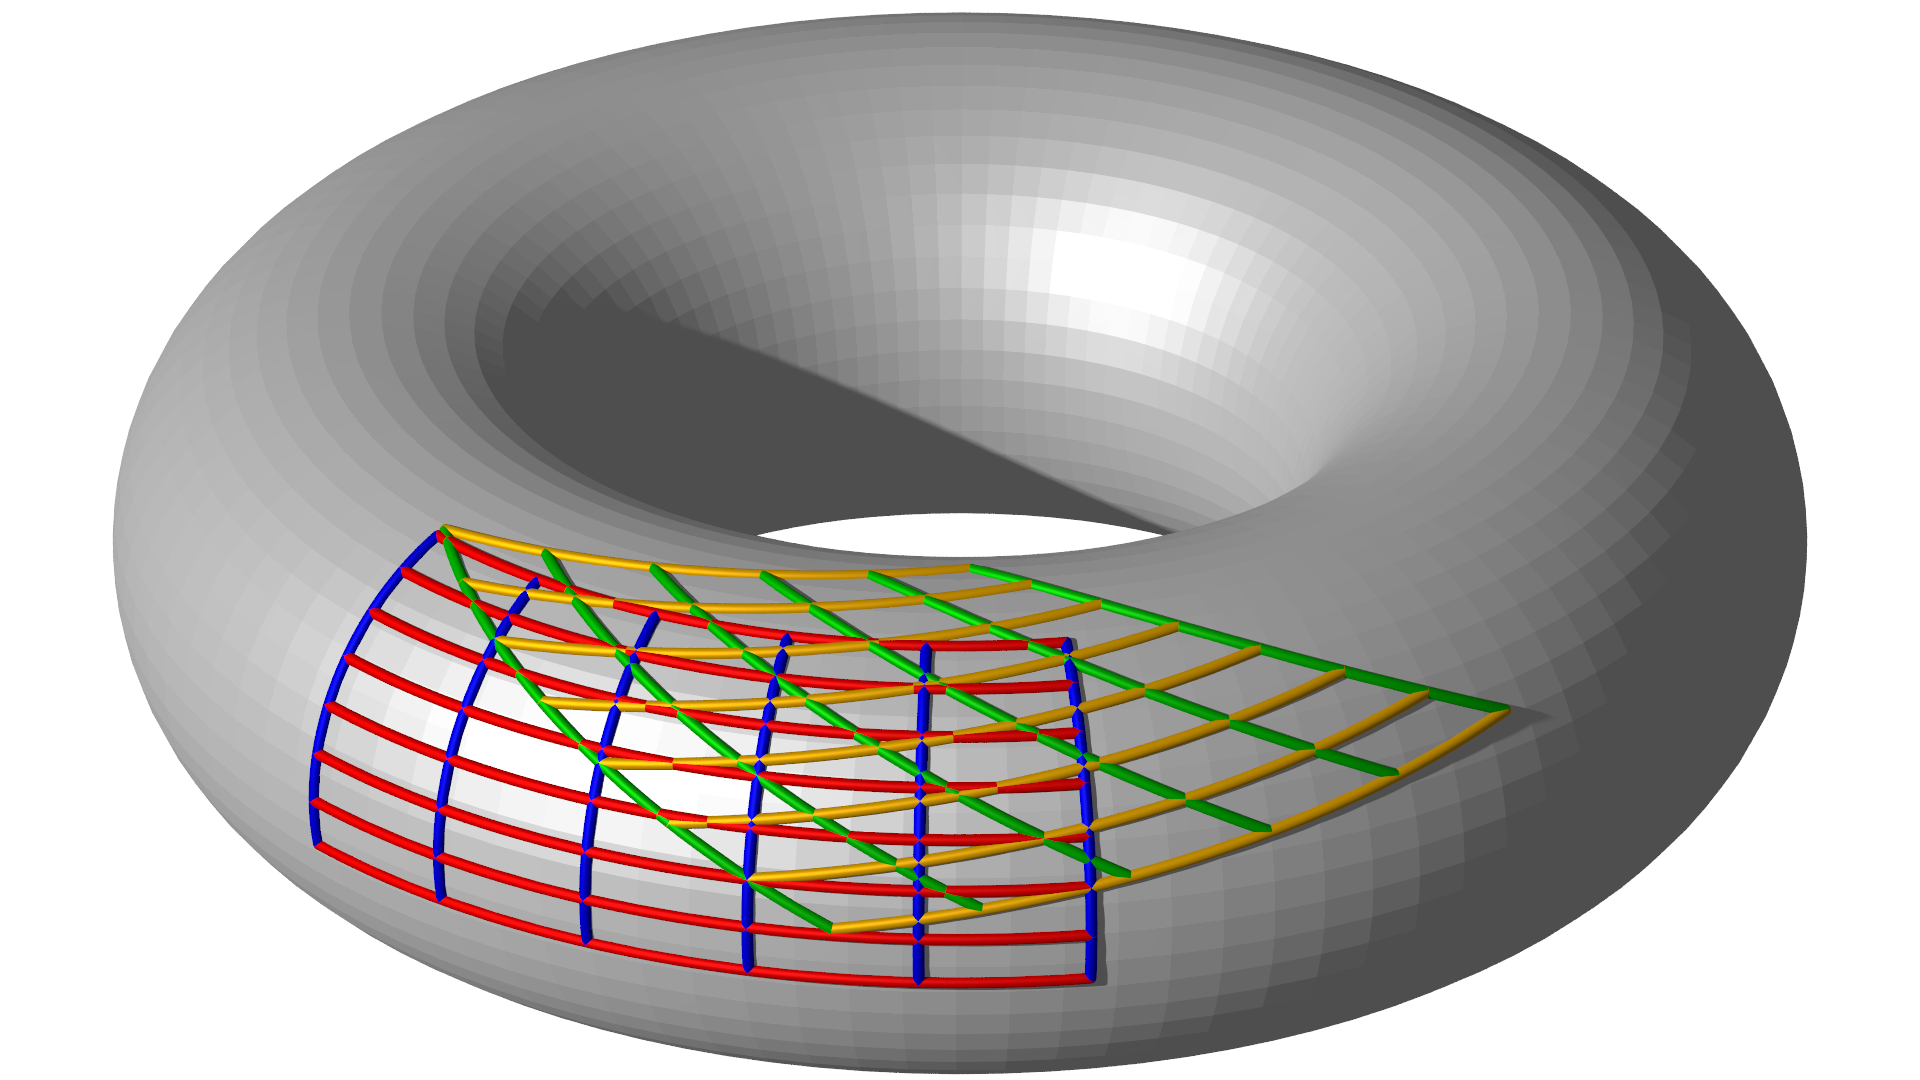
\includegraphics[width=10cm]{torus.png}};

\def\s{3}

\node at (-3.5,-0.4) {$U_\alpha$};
\node at (2.0,-0.4) {$U_\beta$};

\draw[->] (-2,-2.2) -- (-3,-4.3);
\node at (-2.5,-3.25) [left] {$\varphi_\alpha$};

\draw[->] (1.4,-1.7) -- (3,-4.3);
\node at (2.5,-3.25) [right] {$\varphi_\beta$};

\begin{scope}[xshift=-4.5cm,yshift=-8cm]
	\begin{scope}
		\clip (0,{-0.2*\s}) rectangle ({1*\s},{1.2*\s});
		\begin{scope}[xshift=1.8cm,yshift=0.6cm,rotate=30]
			\fill[color=gray!20]
				(0,{-0.2*\s}) rectangle ({1*\s},{1.2*\s});
			\foreach \x in {0,0.2,...,1}{
				\draw[color=darkgreen]
					({\x*\s},{-0.2*\s})
					--
					({\x*\s},{1.2*\s});
			}
			\foreach \y in {-0.2,0,...,1.2}{
				\draw[color=orange]
					(0,{\y*\s})
					--
					({1*\s},{\y*\s});
			}
		\end{scope}
	\end{scope}

	\foreach \x in {0,0.2,...,1}{
		\draw[color=blue,line width=1.4pt]
			({\x*\s},{-0.2*\s}) -- ({\x*\s},{1.2*\s});
	}
	\foreach \y in {-0.2,0,...,1.2}{
		\draw[color=red,line width=1.4pt]
			(0,{\y*\s}) -- ({1*\s},{\y*\s});
	}

	\draw[->] ({\s*(-0.1)},0) -- ({1.1*\s},0) coordinate[label={$x_1$}];
	\draw[->] (0,{-0.3*\s}) -- (0,{1.3*\s}) coordinate[label={left:$x_2$}];

	\node at ({1*\s},{1.2*\s}) [above right] {$\mathbb{R}^2$};

\end{scope}

\begin{scope}[xshift=1.5cm,yshift=-8cm]
	\begin{scope}
		\clip (0,{-0.2*\s}) rectangle ({1*\s},{1.2*\s});
		% x = - [ (sqrt(3)/2)*0.6+(1/2)*0.2 ] = -0.6196
		% y = - [ (-1/2)*0.6 + (sqrt(3)/2)*0.2 ] = 
		\begin{scope}[xshift=-1.8588cm,yshift=0.3804cm,rotate=-30]
			\fill[color=gray!20]
				(0,{-0.2*\s}) rectangle ({1*\s},{1.2*\s});
				\foreach \x in {0,0.2,...,1}{
					\draw[color=blue]
						({\x*\s},{-0.2*\s})
						--
						({\x*\s},{1.2*\s});
				}
				\foreach \y in {-0.2,0,...,1.2}{
					\draw[color=red]
						(0,{\y*\s})
						--
						({1*\s},{\y*\s});
				}
		\end{scope}
	\end{scope}

	\foreach \x in {0,0.2,...,1}{
		\draw[color=darkgreen,line width=1.4pt]
			({\x*\s},{-0.2*\s}) -- ({\x*\s},{1.2*\s});
	}
	\foreach \y in {-0.2,0,...,1.2}{
		\draw[color=orange,line width=1.4pt] (0,{\y*\s}) -- ({1*\s},{\y*\s});
	}
	\draw[->] ({\s*(-0.1)},0) -- ({1.1*\s},0) coordinate[label={$x_1$}];
	\draw[->] (0,{-0.3*\s}) -- (0,{1.3*\s}) coordinate[label={left:$x_2$}];
	\node at ({1*\s},{1.2*\s}) [above right] {$\mathbb{R}^2$};
\end{scope}

\draw[<-,color=white,opacity=0.8,line width=5pt] (2.5,-6.5) arc (55:100:6.5);
\draw[<-,shorten >= 0.1cm,shorten <= 0.3cm] (2.5,-6.5) arc (55:100:6.5);

\node at (0,-5.9)
	{$\varphi_{\beta\alpha}=\varphi_\beta\circ\varphi_\alpha^{-1}$};

\end{tikzpicture}
\end{document}

